\documentclass{aa}
%%%% \documentclass {ws-jai}
\usepackage[flushleft]{threeparttable}
\usepackage[varg]{txfonts}
\usepackage{color}
\usepackage{graphicx}
\usepackage{subfig}    %% For generating a grid of figures.
%% \newsavebox\mybox   %% For generating figure captions which wrap at figure 
%% edges.
%% \newlength\myboxlen
%% \newcommand{\figcap}[2]
%% {%
%%   \sbox\mybox{#1}
%%   \settowidth{\myboxlen}{\usebox{\mybox}}
%%   \centering
%%   \usebox\mybox
%%   \hskip \textwidth
%%   \parbox{\myboxlen}{#2}
%% }

\usepackage{bm}
\bibpunct{(}{)}{;}{a}{}{,} % to follow the A&A style
\begin{document}
%%%% \markboth{P.Prasad}{Design and Commissioning of the AARTFAAC All-sky monitor}
\title{Design and Commissioning of the AARTFAAC all-sky monitor}

%%%% \author{Peeyush Prasad  $^\dagger$, \and Folkert Huizinga $^\dagger$ \and John Romein $^\ddagger$
%%%% \and Daniel van der Schuur $^\ddagger$ \and Ralph  Wijers  $^\dagger$}
%%%% \address{
%%%% $^\dagger$Anton Pannekoek Institute, University of Amsterdam, The Netherlands, p.prasad@uva.nl\\
%%%% $^\ddagger$Group, Company, Address, City, State ZIP/Zone, Country\\
%%%% }
%%%% \address{
%%%% $^\dagger$Anton Pannekoek Institute, University of Amsterdam, The Netherlands, p.prasad@uva.nl\\
%%%% $^\ddagger$Group, Company, Address, City, State ZIP/Zone, Country\\
%%%% }

%%%% \corres{$^\dagger$P.Prasad}

%%%% \begin{history}
%%%% \received{(to be inserted by publisher)};
%%%% \revised{(to be inserted by publisher)};
%%%% \accepted{(to be inserted by publisher)};
%%%% \end{history}
%%%% \maketitle
\author{Peeyush Prasad  \inst{1,2} \and Folkert Huizinga \inst{2} \and John Romein \inst{1}
\and Daniel van der Schuur \inst{1} \and Ralph  Wijers  \inst{2}}

\institute{Universiteit  van Amsterdam \and ASTRON, The Netherlands Foundation for Radio Astronomy}

\date{Received <date> / Accepted <date>}

%% Structured abstract
%%%% \begin{abstract}
\abstract {The  Amsterdam-ASTRON Radio  Transients Facility  And Analysis  Center
  (AARTFAAC)  array is  a  sensitive,  all-sky radio  imager  based  on the  Low
  Frequency Array (LOFAR). It generates images of the low frequency radio sky in
  near real-time with spatial resolution of  10s of arcmin, MHz bandwidths and a
  time cadence  of a few  seconds. The image  timeseries are then  monitored for
  short and  bright radio transients. On  detection of a transient,  low latency
  triggers  will  be  generated  for   LOFAR,  which  can  carry  out  follow-up
  observations.   In  this   paper,  we  describe  the   implementation  of  the
  instrumentation, and its capabilities.}
%%%% \end{abstract}

\keywords{Radio Interferometry - Imaging - Radio Transients - Correlators}

\maketitle

\section{\label{sec:Introduction}Introduction}

\begin{itemize}
\item What are celestial transients \\
Transient astronomy deals  with the detection and  characterization of celestial
transients, sources in  the sky whose detectable properties can  change on short
timescales.   These  explosive   events  provide  insight  into   a  variety  of
astrophysics,  ranging from  emission mechanisms  of jets  to properties  of the
intervening  medium [ref].  There is  a rich  history of  the detection  of such
objects  across  wavelength  ranges,  with  each  wavelength  regime  probing  a
different parameter space [ref].

\item Current  state of  radio instrumentation\\
Studies of short  duration radio emission from such objects  has been restricted
to either very  short timescales (milliseconds to seconds, e.g.  Pulsars), or to
comparitively longer timescales (months to  years) primarily due to instrumental
or observational time constraints, the latter  due to the narrow fields of view.
Radio instrumentation is available in broadly two classes; single dish or phased
array  beam  formed   timeseries  characterized  by  high   time  and  frequency
resolution,  fields of  view  of  a few  degrees  but  poor spatial  resolution.
Aperture  synthesis imaging  observations  address the  latter  to provide  high
spatial resolution,  but have  poor time  resolution, typically  needing several
hours of  observation time  to build up  adequate coverage in  the UV  plane via
earth  rotation aperture  synthesis.   The above  classes  roughly translate  to
coherent  (short  timescales)  and  incoherent (longer  timescales)  sources  of
emission.

\item Current state of the science \\
The serendipitous discovery of a new  class of radio transient termed Fast Radio
Bursts  (FRBs) has  galvanized  interest in  the field.  The  detected FRBs  are
characterized by high associated dispersion  measures, high brightness and short
timescales.  They are  non-repeating for  the  most part.  Their unknown  origin
requires  not  only their  discovery,  but  also  rapid  followup over  a  large
wavelength regime to establish emission phenomena and associated parameters.

The last requirement has led to the development of large field of view radio sky
monitors, with an  aim of continuously surveying large parts  of the visible sky
with shallow sensitivity and at high  time resolution. A trigger is generated on
the reliable  detection of  a transient  in close  to real-time,  allowing other
telescopes to carry out follow-up observations.

\item Suitability of low frequency observations \\
<TODO: Paragraph about  transient sources, some stuff about  spectral indices of
coherent emission and  expected class of sources, at what  brightness levels can
we expect to see things (take from Lazio LWA paper).>

<TODO: Paragraph  summarizing the  current state of  knowledge of  low frequency
transients: Stewart NCP transient, other  searches at low freq. Conclusion: Need
for more monitoring.>

\item What is the AARTFAAC \\
The AARTFAAC  radio transient  monitor is  an All-sky  radio telescope  based on
LOFAR. Its goal is to continuously scan  the skies for bright transients, and on
reliably detecting one, to generate a trigger to other telescopes for sensitive,
broad  band monitoring.   It is  a leading  effort among  a group  of new  radio
telescopes  aiming for  detection  of  bursts of  radio  emission by  continuous
monitoring of the low radio frequency sky.  Such telescopes are characterized by
having  moderate   resolution  and  sensitivity  as   compared  to  contemporary
telescopes, but  with extremely wide  fields of  view (typically all  sky), high
availabilities and autonomous calibration and imaging in near real-time.

The  latter requirements  make  their implementations  challenging. The  antenna
elements used to achieve the wide fields of view are typically dipoles, however,
their low individual sensitivities requires  an order of magnitude larger number
of elements in  the array.  Bringing the resulting large  number of data streams
to a  central location, as well  as their correlation for  carrying out aperture
synthesis imaging thus  poses a significant I/O and  compute challenge. Further,
the  wide fields  of  view at  the  sensitivities of  operation  also result  in
direction  dependent  effects  on  the  incoming  signals,  mostly  due  to  the
ionosphere. These pose  a challenge to calibration, especially  when carried out
in an autonomous manner.

Apart  from  its  primary  goal  of  trigger  generation  on  the  detection  of
transients, the telescope products find use in a variety of science cases. These
include  wide  field  ionospheric  monitoring via  apparent  flux  and  position
variations of  calibrator sources, Solar  monitoring, RFI surveying,  LOFAR beam
model validation etc.

\item AARTFAAC as a data transport, reorganization and computing problem.\\

The  wide field  of  views necessary  for  an instrument  like  AARTFAAC can  be
achieved by sampling the sky with wide field dipoles. This, however comes at the
cost  of lowered  sensitivity per  receiving element.   An instantaneously  well
sampled  UV  plane  is  needed  to  generate a  PSF  with  low  sidelobes.  Both
requirements can be  met by spatially spreading a large  number of dipoles.  The
highest sensitivities  can also be achieved  by the coherent correlation  of the
incoming  signal,  requiring  access  to  the nyquist  sampled  signal  at  full
resolution. Such an arrangement then  requires the aggregation of high bandwidth
data from the receiver elements, necessitating a high speed data network.

The incoming  sampled voltages  pass through  various signal  processing blocks,
resulting  in the  generation of  light curves  for sources  in the  image.  The
estimation of spatial coherences requires the reordering of data to make optimum
usage of  compute resources. Thus, the  functioning of the telescope  depends on
the optimization of the data  transport, data reorganization and computing using
available resources.   An advantage of  having an operating model  consisting of
signal   processing  blocks   operating   on  high   resolution   data  is   the
configurability of the telescope into different  observing modes, as well as the
tapping  off of  data from  an upstream  location.  The  latter ability  makes a
piggy-back  instrument like  the  AARTFAAC possible.  An  important resource  to
optimize is the development time for  each data routing or processing block, and
this has been taken into consideration in the AARTFAAC.


In this  paper, we describe  the implementation  of the instrumentation  for the
AARTFAAC  array,  and the  commissioning  of  its various  subsystems.   Section
\ref{sec:aartfaac_array} describes the array and the receiving antenna elements,
its  relationship  with LOFAR,  and  introduces  the  full architecture  of  the
instrument.    Section   \ref{sec:station_hardware}   describes   the   hardware
implementation in  the field which  allows creating a  data path in  parallel to
LOFAR. This  makes AARTFAAC processing independent  of LOFAR to a  large extent.
In Section \ref{sec:gpucorr}, we describe the implementation of a real-time, GPU
based  correlator  for  AARTFAAC,  while  Section  \ref{sec:calim}  details  the
real-time,   autonomous  calibration   and   imaging  implementation.    Section
\ref{sec:acontrol} describes our  control system for the  full instrument, which
also interfaces with LOFAR.  In Section \ref{sec:results} we present performance
metrics of the instrument as a whole.
\end{itemize}

\section {\label{sec:aartfaac_array}The AARTFAAC array}
We  begin by  summarizing the  subsystems of  the LOFAR  telescope relevant  for
AARTFAAC processing in  Section \ref{subsec:lofar}, and then  elaborating on the
scheme for creating a coupled data path for independent processing by AARTFAAC.

\subsection {\label{subsec:lofar} LOFAR telescope architecture}
The LOFAR telescope \ref{} is a new generation radio interferometer covering the
frequency  range from  10-90  MHz using  inverted V-dipoles  known  as Low  Band
Antenna (LBA),  and from 110-240  MHz using Bowtie  dipoles, also known  as High
Band  Antenna (HBA).   The  antenna are  linearly polarized,  being  made up  of
orthogonally  placed  dipoles in  the  E  and H  plane.  The  LBA dipole  has  a
sensitivity pattern  with a 6dB  field of view of  about $120^o$, while  the HBA
dipoles first undergo  an analog phasing within  a 4x4 tile, which  results in a
field  of view  of  about TODO.  Due  to this  restriction,  the AARTFAAC  array
utilizes only the LBA part of the telescope.

The  telescope itself  consists of  a  large collection  of antennas,  spatially
organized into several  'stations', each spread over ~60. The  stations are laid
out in a  dense core: 24 (TODO:  Check) stations within a 2km  radius, while the
long baselines  of stations of  upto a 1000km are  also present. At  the station
level, the  received and conditioned analog  signals from a dipole  are baseband
sampled with a 200MHz clock and  10-bit quantized.(TODO: Check). The signal from
each  polarization  is then  split  into  spectral  subbands  of ~200kHz  via  a
polyphase  filterbank  implementation.   In  the  regular  LOFAR  station  level
processing, the  dipole subbands are  then digitally phased in  hardware towards
the direction of  an astronomical source to  form a station beam,  which is then
transmitted over optical fiber for further interferometric processing with other
stations.

A  schematic  representation   of  the  LOFAR  level  processing   is  shown  in
Figure. TODO

\subsection {\label{subsec:aartfaac}  The AARTFAAC system}
The AARTFAAC  array consists of  12-stations from within  the core of  the LOFAR
telescope, with interdipole distances ranging  from (TODO) within a station, and
a maximum of TODO across stations.  Due  to the requirement of dipole level data
in order to achieve all-sky imaging, the AARTFAAC creates a coupled data path to
an independent processing  architecture, prior to the phasing up  of the dipoles
in the  LOFAR processing  flow. This allows  simultaneous observing  with LOFAR,
leading to high  availability of the AARTFAAC system. A  subset of the available
subbands are  correlated in a dedicated  GPU based correlator in  real-time. The
estimated visibilities  are sent over  TCP/IP to dedicated servers  for carrying
out the autonomous and real-time  calibration and imaging.  The generated images
are further sent to a software  pipeline for the actual detection of transients,
based  on comparison  of the  image timeseries.  A (planned)  trigger generation
subsystem  will publish  reliable triggers  in the  form of  VOEvents [refTODO],
which can be claimed by other telescopes.

\subsubsection {\label{subsubsec:arrayconf} Array configuration}

\begin{figure*}[htbp]
\centering
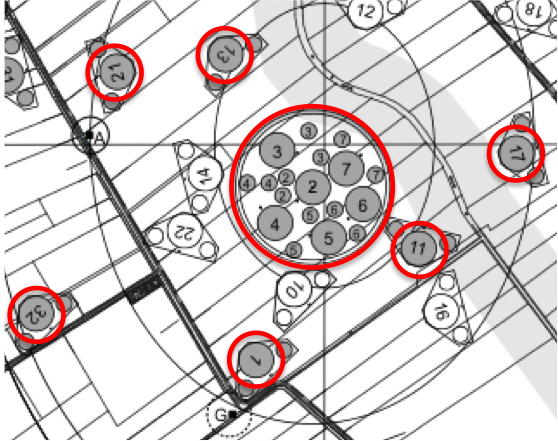
\includegraphics[width=0.25\textwidth]{Figs/afaac12_arrayconfig.png}
\caption{The spatial distribution of AARTFAAC-12 stations within the core of LOFAR stations.}
\label{fig:afaac12_arrayconfig}
\end{figure*}

The choice of stations is dictated primarily by imaging quality and sensitivity,
but  also due  to constraints  on the  latency of  calibration and  imaging. The
central  six stations  of  the LOFAR  telescope (called  the  superterp) form  a
densely sampled UV plane,and are ideal for wide field imaging due to their being
co-planar to  high accuracy (centimeter  level). The outer six  stations provide
higher  sensitivity  and resolution.  The  salient  features of  the  LBA\_OUTER
station configuration  for the chosen stations  are shown in table  TODO. Figure
\ref{fig:afaac12_arrayconfig}  shows the  LOFAR stations  that are  part of  the
AARTFAAC system.

TODO: Add 12-station beam characteristics, expected confusion noise contribution.

\begin{figure*}[htbp]
\centering
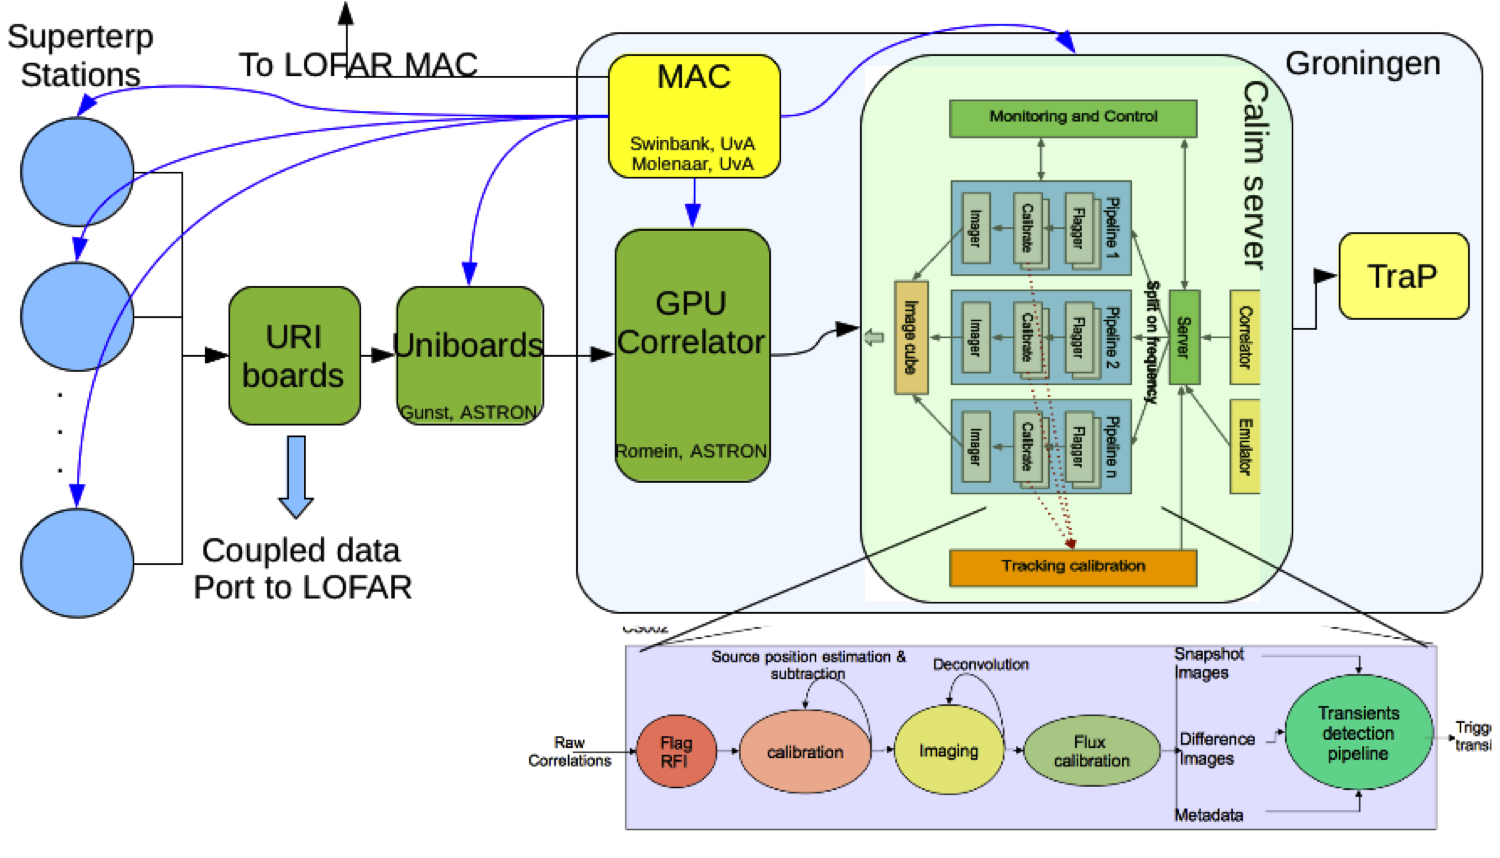
\includegraphics[width=1\textwidth]{Figs/overall_afaac_Arch_blks.png}
\caption{Overall architecture of the AARTFAAC all-sky monitor depicting each processing subblock.}
\label{fig:afaac_arch}
\end{figure*}

The station  consititute the first component  of the radio sky  monitor, and are
the only components shared with LOFAR.  The AARTFAAC monitor consists of further
subsystems which are independent of  LOFAR processing.  Its overall architecture
is shown schematically in Figure  \ref{fig:afaac_arch}, and illustrates the main
processing subblocks of the instrument.   To summarize, a user selectable subset
of subbands  from every dipole  is transferred as  UDP packets over  a dedicated
10Gbit fiber connection  to the central processing systems.   These are received
by  a streaming  software correlator  implementation which  aligns the  data and
estimates  the spatial  covariance matrix  between every  pair of  dipoles.  The
generated visibilities  are streamed  over TCP/IP to  a calibration  and imaging
pipeline component  which carries out  autonomous imaging.  The images  are then
analyzed by a software tool (The  Transients Pipeline, TraP), which extracts the
light curves  of sources  within the  image, and  analyses them  for variability
using a number of parameters. The TraP is described in more detail in \ref{}.

The  specifications of  the  AARTFAAC  monitor are  listed  in  Table TODO.   We
describe the  various subsystems making up  the AARTFAAC All-sky monitor  in the
following sections.

\section {Remote Station Level Processing:} 
Remote  Station processing  refers  to instrumentation  installed  in the  field
coupled to the receiving antennas post balun. This consists of Digital Converter
Unit (DCU)  boards and the  Remote Station  Processing (RSP) boards.  The former
caters to analog  signal conditioning of the received voltage,  followed by base
band digitization  at 200MHz, with TODO bit resolution.\\

The RSP boards handle the reception of  sampled voltages from the DCU boards and
their first stage  processing. In the following, we describe  the parts relevant
to  the functioning  of  the  AARTFAAC telescope.   The  RSP  board consists  of
TODO_NUM TODO_TYPE  FPGAs, with  TODO input bandwidth  over TODO  connector, and
TODO output bandwidth  over TODO connector.  [TODO Add  reference] describes the
implementation of this board  in more detail. A single RSP  board can handle the
processing of sampled data from 4 dual polarized dipoles.  Since a LOFAR station
is made up of 48 dual polarized dipole antennas, 12 such boards are required per
station.\\

\textbf {Signal processing:} The RSP board  carries out the first stage polyphase
filter bank  implementation common  to the LOFAR  and AARTFAAC  telescopes. This
filter bank  analyzes the voltage timeseries  sampled at 200 MHz  available from
the samplers, into a complex voltage spectrum of 512 subbands. The output, for a
set of  1024 real voltage  samples, consists of  fixed point complex  values per
subband. These  values fundamentally have  a 16-bit  resolution on the  real and
imaginary components. [Add some more on dynamic range expected etc.]\\

Station level  beamforming in  a particular  direction requires  calculating the
weighted sum of  all dipoles of the same polarization,  with the applied weights
being dependent on  the direction of beamforming.  Each  RSP board fundamentally
generates the  beamformed product for  its 4  client dipoles for  every subband.
These are termed  as 'beamlets'.  The necessary exchange of  beamlets with other
RSP boards to  create the station beam is achieved  via the interconnect between
the various RSP boards.

\textbf  {Interconnect:}  A  ring  network   consisting  of  four  10-GigE  links
interconnects    the    RSP   boards    to    each    other,   as    shown    in
Fig. \ref{fig:afaac_station_hw}.  It carries beamlet  data, and has  an AARTFAAC
specific  mode (enabled  only  on AARTFAAC  boards? TODO  check)  where the  raw
subbands  for every  dipole  polarization  are also  transferred  onto the  ring
network. Of the total TODO bandwidth of the ring network, about TODO is occupied
by  LOFAR specific  products. The  remaining  bandwidth carries  the per  dipole
subbands, which are used exclusively for AARTFAAC processing.\\ 

The fundamental limitation  to AARTFAAC processed bandwidth is  presented by the
interconnect, and  depends on  the bit-mode chosen.  The bandwidth  available to
AARTFAAC is limited  to 36 subbands in  16-bit mode, 72 subbands  in 8-bit mode,
and 144 subbands in 4-bit mode.

\textbf  {Available bit  modes:}  The system  offers the  ability  to trade  off
dynamic range in  the polyphase filter bank outputs with  the number of subbands
available  for further  processing.  This  is done  by  reducing  the number  of
allocated bits  to the  real and  imaginary components  of the  subband outputs,
leading to an increased number of subbands.  The bit mode of AARTFAAC can be set
completely independently of  LOFAR's choice of bit mode. The  choice between the
various bit modes  depends on the RFI environment of  the observation.[TODO: How
  is the  data converted  from 16-bit to  8-bit? Which 8-bits  are taken  as the
  output?  Implications?].  An  8-bit complex  representation of  the filterbank
outputs  is found  to be  adequate for  almost all  observing conditions  except
during severe RFI.

\textbf {Sampling  clock and Timing:}  A clock  distributer board [TODO  REF] is
used  to  distribute  a  10MHz  reference  to  every  one  of  the  12  AARTFAAC
stations. This  reference is  generated by a  GPS discplined  Rubidium frequency
standard. This ensures that an identical  (hence coherent) clock is used for the
sampling of data from the AARTFAAC stations.\\

Every station is equipped with a Local  Control Unit (LCU), which is an embedded
(TODO:Check?)  processor  running a Linux  operating system.  These  systems are
networked to the LOFAR control system, and  also act as NTP clients. Thus, their
absolute times are aligned to better than a few milliseconds. This absolute time
from the station LCU is communicated to  the RSP board [TODO: Check?] on station
reset, as the  reset value to a  64bit counter.  Once set,  the station hardware
updates  this counter  on a  derivate of  the available  200MHz reference,  thus
ensuring that  the absolute  time is  embedded in the  data with  few nanosecond
[TODO check] resolution. All further aligning and timing of the incoming data is
carried out based on this embedded timestamp.

\textbf {Subband data format:}

\textbf {The Uniboard-RSP Interface board:}

\textbf {The Uniboard based data router:}

\textbf {Control interface:}

\begin{figure*}[htbp]
\centering
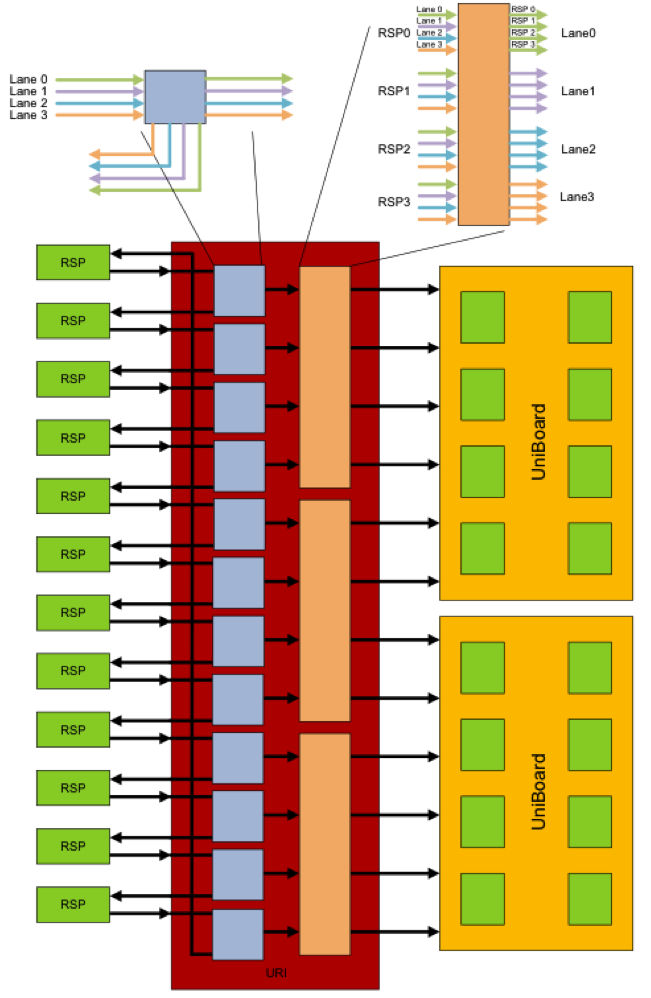
\includegraphics[width=0.75\textwidth]{Figs/station_hw_proc_afaac.png}
\caption{The station level hardware changes  allowing creation of a coupled data
  path for AARTFAAC data flow.}
\label{fig:afaac_station_hw}
\end{figure*}

Figure \ref{fig:afaac_station_hw} depicts the  station level ring network, whose
bandwidth is shared between the beamformed  subbands as well as the dipole level
subbands. The ring network bandwidth constrains the processed AARTFAAC bandwidth
to a fundamental maximum of 64 4-bit subbands, or about 12MHz. The URI boards in
combination with  the uniboards  carry out  a first level  of the  incoming data
transposition.


\subsection {\label{subsec:impact_lofar} Impact of sharing dipoles with LOFAR on AARTFAAC}
LOFAR operates using either  the LBA or the HBA antenna at  a time. Further, due
to limited station level electronics for stations within the core, only a subset
of the available station dipoles can be utilized. This implies that the AARTFAAC
telescope  is  dependent  on  LOFAR  for  the  choice  of  antenna  and  station
configuration,  reducing the  availability  for all-sky  monitoring. Within  the
station, only the LBA\_OUTER station configuration is currently deemded suitable
for  real-time imaging.   This mode  of  LOFAR operation  favorable to  AARTFAAC
depends on  the observing  schedule and the  proposed observations.   Table TODO
shows some  statistics from previous cycles  on the fraction of  observing modes
favorable to AARTFAAC. Based on this, it  may be resonable to expect AARTFAAC to
operate TODO fraction of time, typically.

\section {\label{sec:station_hardware} Station level hardware for piggy-back operation}
\begin {itemize}
 \item {URI board  description, data coupling scheme,  constraints on achievable
   bandwidth}
 \item  {The uniboard  data  reformatting (transpose),  uniboard data  transfer,
   output data format}
 \item {Available diagnostics, performance, commissioning tests}
\end{itemize}

\section {\label{sec:gpucorr} The AARTFAAC real-time correlator}
\begin{figure*}[htbp]
\centering
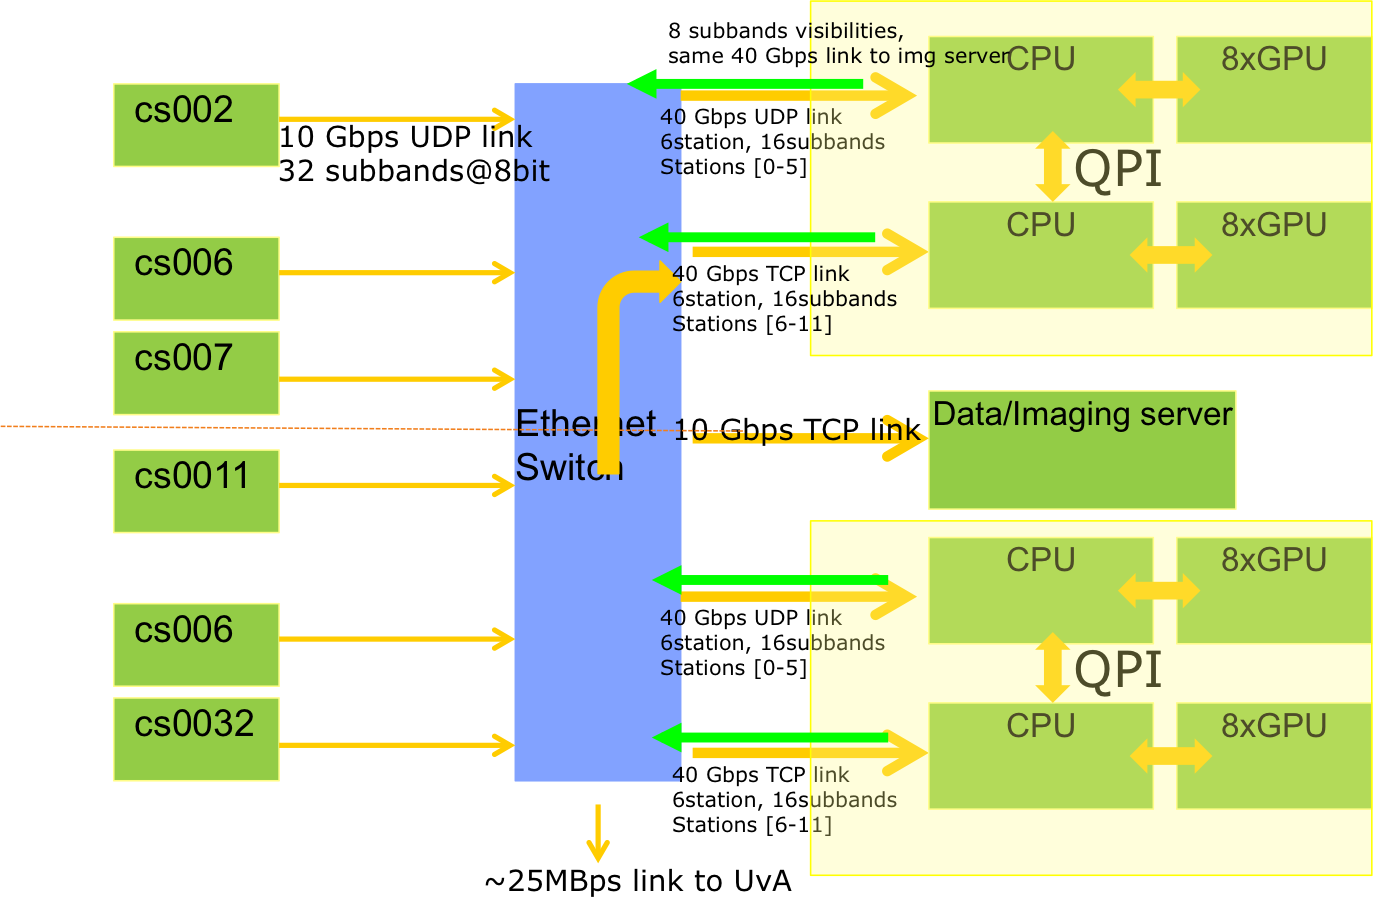
\includegraphics[width=1\textwidth]{Figs/correlator_arch.png}
\caption{The GPU correlator implementation using a pair of AMD(?) CPUs hosting AMD GPUs}
\label{fig:afaac_station_hw}
\end{figure*}
The correlator subsystem  estimates the spectral coherence between  all pairs of
the 1156  polarizations of  the drooped  dipoles, per subband.  This is  done by
computing  the  average  cross  correlation  between  antenna  polarization  per
subband. Its  input is formed of  the subbanded complex voltage  timeseries from
each  polarization  of  every  antenna.  The output  consists  of  a  stream  of
visibilities with a chosen time and frequency averaging.

Correlators have a high input bandwidth and compute requirement, with a low compute per byte footprint. In the recent past, 

- Enormous I/O  requirements. Is a  streaming, real-time application  with large
- I/O  requirements. This  can  be a  problem for  implementation  in many  core
- hardware.   
- Computational demands  grow  quadratically. Challenging  computing step, since  
  computation grows  quadratically with  number of  inputs.
- Recent trend is to correlate in software  instead of hardware, due to flexibility and
- to reduce development effort.
- I/O requirements: 1156*8*16*195312.5 bits/sec.
- Output resolution: Limited by time and frequency smearing effects, described more in a forward section.
- Justification for correlating on a GPU as against special purpose hardware, or super computers (take from a GPU paper).
- Logical blocks of the correlator:
The correlator consists of the following logical blocks:
- The input section: Job is to receive the incoming data.
- The ring buffer for alignment of input streams: Forms a time aligned set of input data. All incoming data packets are copied into a slot in memory based on the timestamp from the data.
- A second level polyphase filterbank is applied to the incoming subbanded data. This provides the necessary input frequency resolution, and also allows to carrout the subband amplitude modulation caused as a side effect of the first stage poly-phase filter bank. The correction is based on a theoretical response to the PFB.
- The input is then passed on to the GPU via a host-device transfer, to carry out the actual correlation. The host-device transfer is on the critical path from latency and throughput perspective.
- The combination of two stations is called a baseline, total number of baselines is N*(N+1)/2. This includes autocorrelations.
- The correlator can operate on different input data modes. We describe the results in terms of 16-bit complex inputs. We address the question of scaling up the system in section [forward ref].
- Description of the operation of correlation.
- Description of the output products.
- Choice of doing floating point operations (get info from e.g. D'Addario)
- How many FLOPS/byte of incoming data? (arithmetic intensity).
- Memory organization in host memory.
- Memory organization in device memory. Any optimizations for reduction of memory loads.
- Tuning of tile size to implementation architecture. Make the tilesize as large as possible while fitting in registerspace for maximum utilization of loaded data.
- Description of tile selection of data and resulting arithmetic intensity.
- Table of properties of the chosen architecture (like table 3 of van niewpoort and romein, many core correlator architecture.)
- Ratio between FLOPS and Bytes/sec of memory bandwidth: indicator of performance of memory system.
- Performance is bound both by theoretical peak performance, and the product of memory bandwidth and arithmetic intensity.
- Mention theoretical peak performance, get teh actual value from John Romein (See Sec. 3.6 of Nieuwpoort paper), what fraction of peak performance is achieved?
- Kernel performance?
- Achieving GPU theoretical performance depends on setting up an adequate tile size, this in turn depends on the nnumber of available registers, and the host-device bandwidth (?).

-- Code related summary points --
- Overall program architecture: What does the CPU do, what gets offloaded to the GPU?
- What tile size is used?
- Are the XY and YX hands calculated? What does -m9 do?
- Buffer sizes, memory footprint?


\begin {itemize}
 \item {Correlation for transit mode observations: logical blocks.}
 \item {Description of processing flow.} 
 \item {Motivation of chosen architecture for implementation.}
 \item {Supported time and frequency binning, motivation of choice.}
 \item {Required compute and memory bandwidth.}
 \item {Synchronization of incoming data (input buffer), output data format.}
 \item {Commissioning tests, performance.}
\end {itemize}

\section {\label{sec:calim} Real-time calibration and imaging}
\begin {itemize}
 \item {Architecture, implementation choices, performance}
 \item  {Visibility  and  image  buffering strategy  for  followup  analysis  of
   detected transients}
 \item {Quicklook images data path}
 \item {Unit test architecture}
 \item {Interface to TraP}
\end {itemize}

\section {\label{sec:acontrol} The AARTFAAC control interface}
\begin{figure*}[htbp]
\centering
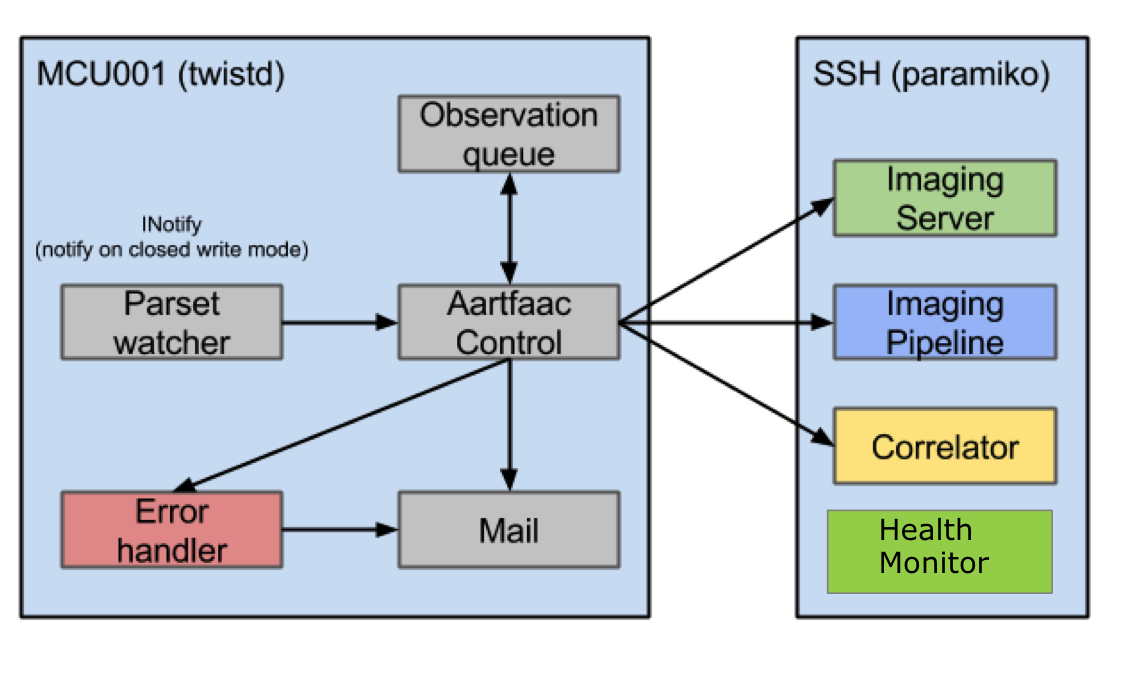
\includegraphics[width=0.25\textwidth]{Figs/control_sys.png}
\caption{The  control  system  architecture  which  interfaces  with  the  LOFAR
  observation scheduling system and triggers AARTFAAC observations.}
\label{fig:afaac_ctrl_sys}
\end{figure*}
Figure  \ref{fig:afaac_ctrl_sys} shows  the  functional blocks  of the  AARTFAAC
control system, and their interface to the LOFAR scheduling system.
\begin {itemize}
 \item {Control system description}
 \item {Interface with LOFAR}
 \item {Monitoring interface: AARTFAAC webpage}
\end {itemize}

\section {\label{sec:results} Commissioning results}
\begin {itemize}
 \item {Overall latency of the system}
 \item {Long term performance of the entire system based on logs.}
 \item {Performance  in various  bit-modes, with  different number  of subbands,
   expected sensitivity.}
 \item {Imaging quality Vs. latency: 6 station to 12 station.}
\end {itemize}

\section {\label{sec:discussion} Discussion}
\begin {itemize}
 \item {Long term operations of the instrument.}
 \item {Triggering mechanism: VOEvents?}
 \item {False alarms (?): Known sources of transients}
 \item {RFI situation}
\end {itemize}

\section {\label{sec:conclusion} Conclusions}

\begin {acknowledgements}

This work  was funded  by the ERC  grant <num> awarded  to Prof.   Ralph Wijers,
Universitiet  Van Amsterdam.   We  thank The  Netherlands  Foundation for  Radio
Astronomy  (ASTRON)  for support  provided  in  carrying out  the  commissioning
observations.
\end{acknowledgements}
\bibliographystyle{aa}
\bibliography{ref}

\end{document}
